\documentclass[authoryearcitations]{UoYCSproject}
\author{Caleb J. H. Riley}
\title{Evolutionary agent-based simulation modelling of human life-history evolution}
\date{Version 0.01, 2016-November-15}
\supervisor{Daniel W. Franks}
\BEng

\wordcount{2001}

\includes{}

\excludes{}

\abstract{This is an abstract. Should be about 500 words long.}

\dedication{}

\acknowledgements{}

\usepackage{framed}
\usepackage{array}
\usepackage{hyperref}
\usepackage{enumitem}
\usepackage{lscape}
\usepackage{listings}
\usepackage{graphicx}
\graphicspath{ {images/} }

\begin{document}
\maketitle
\listoffigures
\listoftables

\cleardoublepage

\chapter{Introduction}
\label{cha:Introduction}
\section{Motivation}
The senescence of organisms is a long standing evolutionary puzzle: why would genes which cause an organism to degrade over time be selected for? In particular, why could genes which cause a reduction in fertility with age provide evolutionary benefit versus reproducing until death? Menopause is of particular interest since it both only occurs within females, but within limited number of species.

Although we know the the biological cause of menopause, there are many theories about why it is beneficial for a species to cease reproduction long before death. This report focuses on the Patriarch Hypothesis, the idea that older male's preference for younger females cause menopause to evolve. 


\section{Aims}
\subsection{Provide an overview of the origin of menopause}
Menopause has many different theories for its origin, and it would be useful to explore some of them as well as contextual information before focusing on the Patriarch Hypothesis in particular.


\subsection{Check validity of computational model}
This project focuses on reproducing a computational model \cite{mateChoice2013} that implements the patriarch hypothesis \cite{patriarchHypothesis2000}, a theory that males' preference for younger females caused long post-reproductive lifespans. Replicating models is useful to check their validity and discover any flaws they may possess. Replication also provides a jumping off point for improving the model or for adapting it to other hypotheses to do with the evolution of menopause or population modelling in general. 

\subsection{Rewrite model into an object oriented language}
The model is also being adapted from C, a performant but verbose and old imperative language, into Python, a modern object oriented language designed to be as readable as possible. Python is also popular among scientific research, so this will make the model more accessible for future work. Object oriented languages are also well suited for making multi-agent systems as the object-attribute-method structure is a good match for modelling the agent, its traits and the ways it can interact with the environment

\subsection{Extend the model to allow co-evolution of preference}
Whilst mortality and fertility are both able to evolve under the current model, the mating preferences of the males are fixed. Since the hypothesis relies on the preference of older males for younger females, it would be useful to see how allowing this preference to evolve over time would affect the results of the model.

\section{Thesis Outline}
\begin{description}

\item[Chapter Two Literature Review] The literature review provides a critical overview of different hypotheses for the origin of menopause, as well as background information on evolution and modelling in biological contexts.
\item[Chapter Three Problem Description] Is an overview of the model that already exists, how it models the hypothesis and shortcomings with the model.
\item[Chapter Four Design and Implementation] Is a description of how the solution to the problem was designed and implemented.

\item[Chapter Five Results and Evaluation] Presents the results of the model created and takes a critical look at how the work progressed.

\item[Chapter Six Conclusion] making judgement of the solution and the results, suggesting new work.

\end{description}

\section{Statement of Ethics}
The project is implementing a computational model which is purely theoretical. Although it concerns human reproduction, it does not involve human subjects and implementing it with them would be impossible due to time constraints (as evolution take place over many many years), there are no real ethical concerns.

\chapter{Literature Review}
\label{cha:Literature Review}
The literature review provides an overview of existing work surrounding the problem, as well as background information that will be relevant to its solution. 

\section{Menopause}
Menopause is the process where females cease having menstrual periods and become infertile. Whilst reduction in fertility with senescence is not uncommon among species, the long lifespan after menopause (post-reproductive lifespans, or PRLSs) are a relatively rare trait, being only found in the wild in humans, short finned pilot whales and orcas (killer whales). Although we understand to some extent the physiological cause (a decrease in oestrogen and progesterone), the evolutionary benefits of a reduction in reproduction seem unclear as any reduction in fertility would seem to be a reduction in evolutionary fitness. As such this evolutionary puzzle has resulted in many different theories for its existence \cite{evolutionPRLS2015}.  

\subsection{Patriarch Hypothesis}
The patriarch hypothesis \cite{patriarchHypothesis2000} hypothesises that menopause came about due to older, high status males having access to younger female mates allowing them to reproduce for much longer. This increased the proliferation of genes linked to longevity, increasing both the lifespan of males and females. This is reliant on several factors: 

\begin{itemize}
\item That females have a limited number of oocytes (immature ova) which are depleted over time, and that reproduction naturally comes to an end when they run out. \cite{humanPopBio1994} In early females, before female longevity increased, most females died before their supply of oocytes had been completely depleted, and so did not experience menopause.
\item That longevity causing mutations are on the X rather than the Y chromosome. If the gene were on the Y chromosome then the increase longevity would only be present in the males. The paper suggests that female longevity (and therefore have long post reproductive lifespans) is a result of females being "dragged along" by male longevity being passed on through the X chromosome. 
\item That older men continue to reproduce and pass on their longevity causing genes. High states males (normally those with a better reputation for hunting and gathering) would start a new family with a second, younger wife once their first wife had undergone menopause. Thus males carrying longevity causing genes would have greater opportunity to pass them on.
\end{itemize}

A mathematical model of the hypothesis was created \cite{whyMenMatter2007} which was a set of functions which relied on a group of females aged i, and a group of males aged j, the females' fertility at age i and the mating preference of females of age i for males of age j and vice versa. The main problem with this model is that it had a fixed age at which females stopped reproducing, rather than letting it evolve over time as you would expect in an evolutionary model. Indeed this model can be interpreted to suggest that males' preference for younger females came to be after the evolution of menopause, rather than as a cause of it.

To try and correct some of these shortcomings, a computational model \cite{mateChoice2013} which does not have a fixed age where females become infertile. Each member of the population is modelled as an individual agent, with genes that affect either mortality or fertility, with genes acting either in a sex dependent or a sex indifferent manner. Pseudo-random numbers are used to determine births, deaths and partnerships against predetermined tables which are modified by genetics. One of the main shortcomings of the model is that it does not allow the preferences of the agents to coevolve with the change in fertility and mortality. 

Overall the main issue with the patriarch hypothesis is that males' preference for younger females may itself be an epiphenomenon which emerged as a result of menopause, rather than the other way round. Knowledge that females would become infertile after a certain age would cause males to have a preference for younger females who had more fertile years left.

\subsection{Grandmother Hypothesis and the Mothering Hypothesis}
The grandmother hypothesis \cite{grandmother2000, grandmotheringProbabilistic2014, longevityGrandmother2012} theorises that the evolution of menopause came about due to the increased inclusive fitness of a population caused by grandmother being able to help her children raise their offspring through providing childcare and resources such as food. This is due to the grandmother being post-reproductive and not having any children that are of an age where they need care. This grandmothering improves the survival of grandchildren and allows her children to reproduce more frequently. Populations which had post-reproductive women would grow more rapidly as a result, meaning they would overtake populations where they did not occur. 

One of the criticisms of the grandmother hypothesis is that the degree of increase to inclusive fitness has been overstated, and that whilst the benefit might be a factor, it is unlikely to be the only factor to have caused it. Another criticism is that if the benefits of grandmothering are so great, why do males remain reproductive throughout their lives? If the increase to inclusive fitness is so great from grandmothering then it seems unlikely that this benefit would be limited to just one sex.

The mothering hypothesis is a similar theory in which a species improves the survival of offspring by ceasing reproduction at a certain point so that resources could be focused on raising existing children, rather than continuing to focus on reproduction and newborn children. The reduced mortality rate of children would again result in an increase of inclusive fitness.

\subsection{Reproductive Conflict Hypothesis}
The reproductive conflict hypothesis \cite{cant2008reproductive, repConflictOrca2017} is another hypothesis based on grandmothers: this time instead of them stopping reproduction to provide childcare, they cease reproduction so that their offspring are no competing for resources such as food with their grandchildren. Menopause reduces the amount of time where a mother is fertile at the same time as her offspring, reducing the likelihood that they have young children at the same time. This reduced competition for resources means that children will have a greater chance of survival, increasing the inclusive fitness of the group as a whole.

\subsection{Other Hypotheses}
A non-adaptive hypothesis is that women have a fixed number of oocytes (immature eggs), and that menopause did not evolve, but is an epiphenomenon of us now living past the age where the they run out. \cite{van2003ovarian, cooper1998age} Proponents of this theory often use the evidence of menopause occurring in some primates in captivity -- their increased lifespan means they now live well past becoming infertile. They suggest that human's improvements to medicine and nutrition have extended our lifespans in the same way, which is why humans now experience menopause. Counter to this however is the fact that menopause is experienced by orcas and short-finned pilot whales. Since they do not have access to healthcare, you can only conclude that although improved lifespan makes a woman more likely to life through menopause, it is not itself what causes it.

Another hypothesis is that menopause came about to guard against the negative effects of pregnancy at an advanced age. Increased maternal age can result in: miscarriage, chromosomal abnormalities, and pregnancy diabetes, among other effects \cite{cleary2005impact}. These complications would result in an increased need for investment of resources in reproduction itself (with a chance that the baby would not make it to full term), as well as resulting in the mother's other offspring being left with fewer resources such as food and childcare, or potentially being left motherless. However the improvements made to medical care have had a greater impact on both infant and maternal mortality, and the effect is a steady increase with age, rather than a sharp threshold effect. This improvement to healthcare came about after menopause was present in humans, and so this cannot be the cause.

\section{Evolution}
Charles Darwin's theory of evolution, first proposed in On the Origin of Species \cite{origin1859} may be one of the most important and influential academic pieces of work in science. The theory supposes that organisms with traits favourable to their environment were more likely to survive and reproduce, increasing the prevalence of the trait over other less useful traits. This is often summarised as "survival of the fittest".

\subsection{Key Concepts of Evolution}
\begin{description}[style=nextline]

\item [Fitness] Fitness is the measure of how well suited an organism is to an environment, and how likely it is to pass on its genetic information as a result. Note that "fitness" in this instance is relating to how well an organism "fits in" with its environment, and not athletic fitness.

\item [Inclusive Fitness] Inclusive fitness is an extension of the concept of \textbf{Fitness}, in which you can improve your fitness by improving the survival of individuals with similar genetics to you, such as siblings, nieces and nephews or grandchildren. This increase to fitness is proportional to your relatedness to them. Improvement of inclusive fitness could come about due to provision of resources such as food and childcare.

\item[Selection] Selection is the process in which survival and reproduction of a species is affected by the phenotype (physical expression of genetics). A trait that increases lifespan and allows more time for reproduction will cause there to be a greater chance for more offspring with that trait to be produced. By comparison a trait that decreases lifespan or realised fertility will tend to become less prevalent in the population as they have fewer offspring and these offspring if they have the same phenotype will inherit the lower survival chances. In essence useful traits survive, whereas traits that are less useful will gradually disappear.

\item [Crossover] Crossover is part of the process that combines the genetics of two parents into the new set of genetics present in their offspring. For each chunk of genetic information, the offspring has a 50\% chance of receiving that information from their mother, and a 50\% chance of receiving the information from their father. This result in an offspring with traits of both their mother and father. When a gene at a particular location is the same in both the mother and father, this gene is transmitted to the child 100\% of the time. 

\item [Mutation] Genetic mutation is the change of genetic information at random, usually from mistakes when copying genes over from their parents. This random change results in the emergence of new traits since it can result in genetics that are not previously present in the population. These new traits can be deleterious, neutral or positive.

\item [Coevolution] Coevolution is the evolution of traits in a species in response to the evolution of traits in the  same or another species. Think of it as a genetic arms race; a species that evolves a form of camouflage may cause a species that predates on 

\end{description}


\section{Modelling in Biology}
In biology, there are many problems that it is only possible to study through the use of modelling. This can be due to the difficulty in finding individuals to study (and therefore a lack of data), the amount of time required to conduct a study (especially for evolutionary effects which take place over many generations) or the ethical constraints of conducting experiments on living organisms (especially humans). Thus models provide a useful tool for examining in a theoretical space hypotheses that cannot be studied in the physical space.

\subsection{Differential Equations}
Differential equations are a traditional tool for use in modelling in general, as they allow you to model the rate of change in a system (using its derivatives). The Verhulst-Pearl equation \cite{garnier1838correspondance, pearl1920rate} in Figure \ref{fig:verhulstPearl} is an old model for simulating population growth. 

\begin{figure}[h]
$$\ \frac{dN}{dt} = rN(1-\frac{N}{K}) $$
\caption{Verhulst-Pearl Equation}
\label{fig:verhulstPearl}
\end{figure}

N is the current population at time \textit{t}, \textit{r} is the rate of population growth and K is the carrying capacity of the system, o the maximum number of individuals the environment it capable of supporting. As N approaches K the rate of population growth slows until an equilibrium is met. Differential equations are capable of modelling complex systems with several variables, but reaching a solution is not always possible. 

\subsection{Multi-Agent Systems}
Multi-agents systems are used to model individuals that interact with each other in a similar way to how organisms interact with each other. Rather than modelling a population through differential equations, you could model it by having a set of agents, who interact to form couples and produced offspring based on their inherent properties such as fertility, mortality and age. The population growth would then become apparent through the emergent properties of the system, rather than through a set, programmed idea.

\begin{framed}
More detail/ideas here. 

References needed
\end{framed}


\subsection{Genetic Algorithms}
Genetic algorithms are mathematical representations of the process of evolution, with the genetics being used to set parameters for program behaviour, rather than the traits of an organism. An initial pool of individual genetics (typically binary strings are used) are created. These gene strings are then used to set parameters for whatever computation is being done. The best performing sets of genes are selected using an arbitrary heuristic fitness function (such as shortest path) to create the next generation of genetics. 

Random parents are selected from the best performers, and the next generation are created by crossing over the genes of the parent pair. The next generation of individuals also undergo random mutation of their genes (i.e. by flipping random bits of the binary string) to prevent the algorithm from getting stuck on a single solution and to produce potentially beneficial genes which may have not appeared in the population yet (and so cannot be acquired from their parents). These stages all correspond to the concepts of biological evolution, and so can be useful when modelling genetic change. Genetic algorithms are good at working out optimal solutions to problems with lots of parameters as the algorithm combines parts of the best solutions from each generation to produces new, potentially better solutions. 

\begin{framed}
More detail/ideas here. References needed
\end{framed}


\chapter{Problem Description}
\label{cha:Problem Description}

\section{Constraints of the Patriarch Hypothesis}
The patriarch hypothesis \cite{patriarchHypothesis2000} states that menopause came about due to older males' preference for younger females. Since humans have relatively long lifespans and the trait of long, post-reproductive lifespans is present in all humans, it is necessary to use a model to study the validity of this hypothesis. In the paper, 3 main conditions that the hypothesis depends on are set out -- it follows that any model examining the hypothesis should model these constraints. The constraints are as follows:

\begin{enumerate}
\item That the depletion of oocytes (undeveloped ovum) must be a constraining factor on when menopause occurs. Menopause was not previously observed until longevity increased to the extent that females lived long enough that depletion could occur.

\item That longevity causing genes are present on the X chromosome, rather than the Y. If it were present on the Y chromosome then a general increase in longevity would only be present in males. Thus the increase in longevity must be on the X chromosome.

\item That older, high status males still reproduce. This is required for the accumulation of a longevity promoting genome, as if a male with genes predisposing him to a long life only reproduces over the same time period as one without the longevity promoting gene (who lives for a shorter time), then they will have an equal chance of passing their genes on and the longevity gene will not become more prevalent.

\end{enumerate}


\section{Why Men Matter: a mathematical model}
A mathematical model was created \cite{whyMenMatter2007} based on the two sex demography work of Schoen \cite{schoen1981harmonic} and Pollak \cite{pollak1990two} which link together a group of females and a group of males of different ages. The marginal fertilities for females and males are constructed in a similar manner (as seen in Figure \ref{fig:marginalFertilities}) but marginal male fertility is assumed to be positive when realised male fertility is non-zero . These marginal fertilities do not represent and individual's virility, rather their biological ability to procreate combined with the chance they are able to mate.

\begin{figure}[h]
$$\ G^F_n = \sum_{ij} \frac{\delta B_{ij}}{\delta F_n}, \qquad G^M_n = \sum_{ij} \frac{\delta B_{ij}}{\delta M_n}$$
\caption{Marginal fertilities of females $\ G_n^F $ and males $\ G_n^F $ }
\label{fig:marginalFertilities}
\end{figure}

These marginal fertilities make up part of the equation for stable growth (Figure \ref{fig:stableGrowth}), where $\ l_n^F $ and $\ l_n^M $ correspond to the female and male life expectancies respectively, and $\ \sigma $ is the male-to-female sex ratio at birth.

\begin{figure}[h]
$$\ 1 = \sum_{n\geq 1}(G_n^Fl_n^F\lambda ^{-n} + \sigma G_n^Ml_n^M\lambda ^{-n}) $$
\caption{Stable growth equation.}
\label{fig:stableGrowth}
\end{figure}


A harmonic mean model similar to that of Schoen's \cite{schoen1981harmonic} was constructed, where $\ b_i $ is the fertility of a female aged \textit{i}, and $\ \alpha_{ij} $ are mating preference weights determined by real world data.

\begin{figure}[h]
$$\ B_{ij} = \frac{b_i\alpha_{ij}F_iM_j}{F_i + M_j} $$
\caption{Harmonic mean model}
\label{fig:harmonicMean}
\end{figure}

When it comes to the three constraints imposed by \cite{patriarchHypothesis2000} this model implements a reduction in female fertility in time but does not specifically link this to the oocyte depletion. The paper does however note that it is important to model the fertility and mortality of both sexes as any mutation that increases mortality past the age of menopause has no effect on population growth when only dealing with females. The model treats this mutation as being sex indifferent (meaning it would have to be located on the X chromosome). For the third constraint the paper largely relies on citing real-world data of hunter-gatherer societies and their social structures as evidence for continued male reproduction later in life. Data from the Dobe !Kung society \cite{howell1979demography} and preconstructed life tables \cite{gurven2007hunter} were used in the harmonic mean model (Figure \ref{fig:harmonicMean}) to this effect.

The main issue with this model is the fixed age of the end of reproduction, as mutations are only used to alter mortality, when they should also be used to affect the fertility of females since the focus of the hypothesis is based on is why menopause in humans came about. Similarly mating preferences of individuals are fixed.

Couples are also not persistent between time steps, which could influence the model since they claim that monogamy is a common social structure within modern hunter gatherers, the hunter gathers they in turn use the data from to drive their model. 

\section{Mate Choice and the Origin of Menopause: a computational model}
Rather than modelling the hypothesis as a complex set of equations, Morton et \cite{mateChoice2013} used an agent-based model. The model creates a random initial population, with random ages and genetics. A population burn-in is performed to generate the inherent age structures of the population by assigning members to random age classes, then causing them to reproduce asexually without the interference of mutations.

After this burn in period, the main simulation begins. First comes the ageing process: each generation, each member of the population has a value from their survival table (modified by mortality affecting mutations) compared to a pseudo-random number to determine whether they are assigned to the next age class or die.

Then comes the reproductive phase. Two random parents from the population are selected. If they are a compatible couple (determined by a preference matrix $\ M_{ij} $ where i and j refer to their age classes) then their fertilities are checked in a similar manner to their survival to determine whether a child is born. This is repeated until all the individuals who died in the ageing process are replaced (keeping the population at a set size). The offspring receives genetic information from their parent and mutations are introduced according to a mutation rate. The model then repeats the ageing and the pairing/reproduction phase for a predetermined number of time periods, logging results as it goes.

The main problem with the mathematical model has been fixed: the age of the end of reproduction is no longer fixed. Since the fertility of an individual is affected by mutations, the fertilities of population as a whole will change over time depending on how fertility-affecting mutations accumulate over time (whether the effects are beneficial or deleterious).

However the fixed mating preferences of individuals remains. With fixed mating preferences the model presupposes the social structures of early hunter-gatherers, justifying this with data from modern hunter-gatherer tribes. The mating preferences of older men for younger females may instead be an epiphenomenon of menopause developing in women -- if realised fertility is the main reason for living then males are far more likely to choose a partner who has more years of reproductive capability ahead of her than one few or none at all. If mating preferences were not fixed we would be able to see if they are stable (meaning they change little regardless of changes in the mortality and fertility of the population) or if they coevolve alongside mortality and fertility changes. If the male preference for younger females evolved from a male preference for female their own age alongside the changes to fertility, this could suggest that the preference came about due to menopause rather than causing it.

\section{A better model}
A better model for the patriarch hypothesis would have the following features:

\begin{itemize}
\item It would generate a typical base population asexually using mortality tables and a burn in period so that correct age structures were created. Starting with these age structures is important to ensure that when the simulation starts there is a variety of ages from which couples can form (or preference based on age would not matter).

\item Each generation, in the ageing phase each member the population is aged or killed on the basis of a pseudo-random number, a mortality table and the presence of mortality affecting mutations in their genes (acting in both a sex-indifferent and sex-dependent manner). The deceased members of the population would then be replaced with new offspring in the pairing and mating phase.

\item Next would come a pairing phase in which couples would form on the basis of a mating preference matrix. Unlike previous models, this preference matrix would be affected by mutations in the genetics of the individual in the same way that mortality and fertility are affected. This would allow the preference to coevolve alongside changes to mortality and fertility.

\item These pairings would also be persistent throughout generations. At present couples are selected from the male and female population pseudo-randomly each generation and checked for mating preference before attempting reproduction if a pairing is formed. Non-persistent unions are inconsistent with the monogamy that the original paper posits as the norm in hunter-gatherer societies. It is unlikely that a male would commit the resources to try and find a new mate if his present partner is still fertile. As such pairings that are persistent between generations (checking to see if mating preference between the pair still exists each generation) is a good model for monogamy, with males only seeking a second mate after the preference for their own partner disappears. The breakup of couples would occur just before the pairing phase, so that new pairings can be formed from the newly single individuals.

\item After the pairings are formed, couples would be pseudo randomly selected from the set of couples and using a pseudo-random number and their fertility distributions (modified by fertility affecting mutations in their genes).

\end{itemize}


\begin{framed}
Existing model overview - relate to code

What has been done

Limitations of their model

How this can be fixed
\end{framed}

\chapter{Design and Implementation}
\label{cha:Design and Implementation}

\section{Class Structure}
When designing a multi-agent system, it can be useful to model each agent as being an instance of a class, each with their own attributes (variables belonging to a class instance that are an abstract representation of the differing traits an agent has) and class methods (representing the actions an agent can take to interact with its environment). The individual people in the system are modelled using the \texttt{Person} class, with attributes determining their traits, including genetics and various probability and preference distributions. 

\newpage
\subsection{Person Class}
The \texttt{Person} class provides the container for the attributes and methods necessary to build the model. Many of its attributes are instances of the classes used to hold probability distributions in control of mortality and fertility, as well as the person's mating preferences and genetics. Each time a new child is born, a new instance of \texttt{Person} is created, with the parameters for \texttt{\_\_init\_\_()} (see Table \ref{tbl:personMethods}) based on their parents' attributes.

\begin{table}[h]
\caption{Person Class Attributes}
\label{tbl:personAttributes}
\begin{tabular}{l l m{5cm}}
\textbf{Attribute} & \textbf{Type} & \textbf{Purpose} \\\hline
\texttt{age} & int & Age of the person \\\hline
\texttt{sex} & str & Sex of person ("f" for female and "m" for male) \\\hline
\texttt{alive} & bool & Whether the person is currently alive \\\hline
\texttt{mortality} & MortalityDistribution & The mortality distribution of the individual. \\\hline
\texttt{reproduction} & ReproductiveDistribution & The mortality distribution of the individual. \\\hline
\texttt{pref\_dist} & PreferenceDistribution & The mating preference distribution of the individual. \\\hline 
\texttt{genes} & Genetics & The genetic information of the individual
\end{tabular}
\end{table}

\begin{landscape}
\begin{table}[h]
\caption{Person Class Methods}
\label{tbl:personMethods}
\begin{tabular}{m{8cm} m{8cm}}
\textbf{Method} & \textbf{Purpose} \\\hline
\texttt{\_\_init\_\_(self, age, sex, mort\_dist, repr\_dist, genes=None)} & Used when instantiating the class, setting up initial values for the properties based on those passed as parameters\\\hline
\texttt{\_\_repr\_\_(self)} & Returns a string representation of the class \\\hline
\texttt{row\_builder(self)} & Returns a list of properties for outputting to csv\\\hline
\texttt{increase\_age(self)} & Assigns a person to next age class if they survive the current generation (based on a pseudo-ransom number and their mortality distribution), otherwise sets \texttt{alive} to \texttt{False}.\\\hline
\texttt{calculate\_age\_class(self)} & Returns the derived attribute \texttt{age\_class} \\\hline
\texttt{reproduce(self)} & Returns \texttt{True} if a person is currently able to reproduce (based on a pseudo-random number and their reproductive distribution). \\\hline
\texttt{calc\_preference(self, other)} & Calculates and returns the mating preference that this person has for the other person (using their ages classes and the person's preference distribution) \\\hline
\end{tabular}
\end{table}
\end{landscape}

\newpage
\subsection{MortalityDistribution Class}
The \texttt{MortalityDistribution} class serves as a lookup table for the probability of death a given age, based on data from the input files \texttt{female\_data.csv} and \texttt{male\_data.csv}. There are two base instances of this class created \texttt{female\_mortality} (using female\_data.csv), the mortality distribution used by females and \texttt{male\_mortality}, for males (using male\_data.csv). The class also contains methods for getting survival probabilities based on age (see Table \ref{tbl:mortalityDistributionMethods}).

\begin{table}[h]
\caption{MortalityDistribution Class Methods}
\label{tbl:mortalityDistributionMethods}
\begin{tabular}{m{0.5\textwidth} m{0.5\textwidth}}
\textbf{Method} & \textbf{Purpose} \\\hline
\texttt{\_\_init\_\_(self, input\_file)} & Used when instantiating the class, reads distribution input from file\\\hline
\texttt{\_\_repr\_\_(self)} & Returns a string representation of the class \\\hline
\texttt{get\_survival(self, age)} & Returns mortality probability value based on age.\\\hline
\texttt{get\_survival\_by\_age\_class( self, age\_class)} &  Returns mortality probability value based on age class.
\end{tabular}
\end{table}

\newpage
\subsection{ReproductionDistribution Class}
The \texttt{MortalityDistribution} class serves as a lookup table for the probability of being able to reproduce at a given age, based on data from the input files \texttt{female\_data.csv} and \texttt{male\_data.csv}. There are two base instances of this class created \texttt{female\_mortality} (using female\_data.csv), the mortality distribution used by females and \texttt{male\_mortality}, for males (using male\_data.csv). The class also contains methods for getting survival probabilities based on age (see Table \ref{tbl:reproductionDistributionMethods} for overview).


\begin{table}[h]
\caption{ReproductionDistribution Class Methods}
\label{tbl:reproductionDistributionMethods}
\begin{tabular}{m{0.5\textwidth} m{0.5\textwidth}}
\textbf{Method} & \textbf{Purpose} \\\hline
\texttt{\_\_init\_\_(self, input\_file)} & Used when instantiating the class, reads distribution input from file\\\hline
\texttt{\_\_repr\_\_(self)} & Returns a string representation of the class \\\hline
\texttt{get\_reproduction(self, age)} & Returns reproduction probability value based on age.\\\hline
\small\texttt{get\_reproduction\_by\_age\_class( self, age\_class)} \normalsize &  Returns reproduction probability value based on age class.
\end{tabular}
\end{table}

\newpage
\subsection{PreferenceDistribution Class}
The \texttt{PreferenceDistribution} class is used to store in the class attribute \texttt{} the mating preferences based on age class of each individual, and to provide access to the data. There are three instances of this class created \texttt{female\_preference} representing females' mating preferences (using data from female\_pref.csv), \texttt{male\_map\_preference} representing males who have a preference for females their own age (using data from male\_map.csv) and \texttt{male\_myp\_preference} representing male preference for younger females (using data from male\_myp.csv). The data is then accessed with the age classes of two individuals (see Table \ref{tbl:preferenceDistributionMethods} for overview).

\begin{table}[h]
\caption{PreferenceDistribution Class Methods}
\label{tbl:preferenceDistributionMethods}
\begin{tabular}{m{0.5\textwidth} m{0.5\textwidth}}
\textbf{Method} & \textbf{Purpose} \\\hline
\texttt{\_\_init\_\_(self, name, input\_file)} & Used when instantiating the class, reads distribution input from file\\\hline
\texttt{\_\_repr\_\_(self)} & Returns a string representation of the class \\\hline
\texttt{get\_preference(self, age\_class\_one, age\_class\_two)} & Returns the mating preference of a person age\_class\_one for a person of age\_class\_two.
\end{tabular}
\end{table}

\newpage
\subsection{Genetics Class}
The \texttt{Genetics} class handles the genetic information of the person, storing it as a string of "1"s and "0"s inside the \texttt{genes} attribute. The class contains a method for generating a random gene string, as well as ones for performing crossover of the genes of two parents and introducing mutations (see Table \ref{tbl:geneticsMethods} for overview).

\begin{table}[h]
\caption{Genetics Class Methods}
\label{tbl:geneticsMethods}
\begin{tabular}{m{0.5\textwidth} m{0.5\textwidth}}
\textbf{Method} & \textbf{Purpose} \\\hline
\texttt{\_\_init\_\_(self, genes=None)} & Used when instantiating the class. Uses genetic string passed or generates random gene string using the \texttt{random\_genes} method.\\\hline
\texttt{\_\_repr\_\_(self)} & Returns a string representation of the class \\\hline
\texttt{random\_genes(self, size)} & Returns a random string of "1"s and "0"s of length equal to \texttt{size}. \\\hline
\texttt{crossover(self, other)} & Returns a gene string made of of random segments of the two gene strings. \\\hline
\texttt{mutate(self, rate)} & Pseudo-randomly flips "0"s and "1"s in the \texttt{gene} attribute with a probability equal to \texttt{rate}.
\end{tabular}
\end{table}

\newpage
\section{Set up and burn-in period}
After the class definitions, the main distributions are set up (female\_mortality, male\_mortality, female\_reproduction, male\_reproduction, female\_preference, male\_map\_preference and male\_myp\_preference) as detailed in their relevant class sections. An initial population of 500 females was created using the premade female distributions, and random ages and genetics. A burn-in period of time (100 generations) is created in which in which they aged and deceased individuals are replaced with new females aged 0, so that a typical age structure based on the mortality distribution is then produced. 

This process is then repeated with the males to produce a male population. The males are all initialised with the male\_map\_preference mating preference distribution since it does not affect this burn in period. Before the actual simulation is run up the preference distribution can be set to male\_map\_preference when males have a preference for females of their own age, or male\_myp\_preference if they have a preference for younger females. 


\begin{table}[h]
\caption{Base population values}
\label{tbl:basePopulationValues}
\begin{tabular}{m{0.2\textwidth} m{0.4\textwidth} m{0.4\textwidth}}
\textbf{Attribute} & \textbf{Female Value} & \textbf{Male Value} \\\hline
\texttt{age} & Random age between 0 and 85 inclusive (multiple of 5) & Random age between 0 and 85 inclusive (multiple of 5) \\\hline
\texttt{sex} & "f" & "m" \\\hline
\texttt{alive} & True & True \\\hline
\texttt{mortality} & female\_mortality & male\_mortality \\\hline
\texttt{reproduction} & female\_reproduction & male\_reproduction \\\hline
\texttt{pref\_dist} & female\_preference & male\_map\_preference \\\hline 
\texttt{genes} & Randomly generated by \texttt{Genetics} class & Randomly generated by \texttt{Genetics} class
\end{tabular}
\end{table}

This initial population is exported to \texttt{initial\_population\_output.csv} and duplicated so that population can then be used for both the simulations.


\newpage
\section{Running the simulation}
The simulation was divided into two phases: the MAP simulation, which models when males have a preference for females their own age, and the MYP simulation, when males have a preference for younger females. The process for each simulation is identical except for the preference distribution of each male. Each simulation set to run for 100 generations (each generation representing a year period) with a mutation rate of 0.2.

The MAP model is run first. Each generation the model starts with an ageing phase. It loops through each female, and assigns them either to the next age or kills them based on a pseudo-random number and their mortality distribution, using the \texttt{increase\_age()} method (see Table \ref{tbl:personAttributes}). This process is repeated for the males.

Next comes a reproduction phase which loops until the population size is restored to 1000. A female and a male are randomly selected from the female and male populations. Their mating preferences are checked and if they are are compatible a mating pair is formed. Then whether they are able to reproduce is checked with both the male and the female. If they are both able to, then a child is produced.

The child's sex is randomly determined with a 50\% chance for a female and \% chance for a male to be born. The child inherits the reproductive, mortality and mating preference distributions of the parent of the same sex. The genetics of the offspring are determined by first performing a crossover of their parents' genes, followed by a mutation with an arbitrary mutation chance of 0.2 (see Table \ref{tbl:geneticsMethods}).

Various statistics about the generation are calculated (including the age distribution of its members) and outputted (see the Generating an output section). The simulation then repeats with the next generation. After all the generations are complete the current population are outputted, then the simulation is repeated using the same method for the MYP model (making sure to change the mating preference distribution for the males).

\newpage
\section{Generating an output}
There is little point to running a simulation if the results are not outputted. The \texttt{csv} module for Python was used both for parsing the input files, but for generating output \texttt{csv} files. The \texttt{csv} format is designed to be a human and machine readable format for storing tables of data and is readable by a variety of programming languages as well as by spreadsheet software, making it an accessible format to output to.

The first thing outputted by the program is the properties of the initial population (using the \texttt{row\_builder()} method - see Table \ref{tbl:personMethods}), outputting the age, sex, life status, genes and preference distribution type to initial\_population\_output.csv. This process was repeated with the populations at the end of both the MAP and the MYP simulations, outputting to map\_population\_output.csv and myp\_population\_output.csv respectively.

The other thing outputted by the program is information about each generation in the simulations. In each generation, the following information is exported: the generation, the number of females, the number of males, the average age of female age of reproduction, the average male age of reproduction, the average age gap in mating pairs who reproduced, the oldest female who reproduced and the oldest male who reproduced. Also outputted each row is the number of individuals in each age group, which allows you to work out the distribution of deaths by age, as well as the number of individuals born each generation. These results are outputted to map\_simulation\_output.csv and myp\_simulation\_output.csv for the MAP and the MYP simulations respectively.

\newpage
\section{Not Implemented}
Unfortunately the work was not completely implemented. The following features were planned, but not implemented:

\begin{itemize}
\item The genetics of a person should affect their mortality. This would be implemented on the MortalityDistribution class by using the person's genetics as well as sex as parameters so that specific loci in a person's genetics could act in a sex-specific or sex indifferent manner to alter their survival. The reason this is important is it provides the advantage to late-age male reproduction over males ceasing reproduction when females do. If there is a mortality-causing mutation that only affects individuals over 55, it will not affect the realised fertility of the females, but males that do not have the mutation will be able to reproduce more, causing this mutation to be selected against.
\item The genetics of a person should also affect their reproduction. Similarly this would be implemented on the ReproductionDistribution class using the person's genes and sex as parameters. This is important for the accumulations of genes deleterious to reproduction in females.
\item The coevolution of the mating preferences of the people. If the mating preferences are not allowed to evolve, then it is difficult to say whether males' preference for younger females caused the evolution of menopause, or the evolution of menopause what what caused males' preferences to come about. 
\end{itemize}


\chapter{Results and Evaluation}
\label{cha:Results and Evaluation}
Since the model was not fully implemented, with genetics being stored and mutated, but these mutations having no effect on fertility or mortality, the results are somewhat limited. Nevertheless some information may be gleaned from the output produced. Presented below are some of the results of a typical run and some analysis of what these results mean. Since the model relies heavily on pseudo-random numbers these results are dependent on one particular run, although the model could be run many times and the results averaged to minimise this effect.

\section{Results of a typical run}
The model was run for 100 generations, with both the MAP (males with a preference for females their own age) and MYP (males with a preference for younger females) using the same base population generated in the burn in period. 

\subsection{Female and Male Numbers}
The base population from the burn in period produces a population with 500 females and 500 males (1000 total). Although the measure of how many females and males there are at any point may not be that useful, it is good to ensure that one sex did not become dominant over the other since this could skew the other results. The population numbers are held at 1000 at all times.

In the MAP model there was a mean of 498.4 female and 501.6 males (with variance $\ \sigma^2 = 276.969 $) with a median of 497 females and 503 males. The minimum number of females reached was 463 and the maximum 545 (range 82), and the minimum number of males was 455, with the maximum 537 (range 82).

In the MAP model there was a mean of 495.36 female and 504.64 males (with variance $\ \sigma^2 = 138.091 $) with a median of 495 females and 505 males. The minimum number of females reached was 459 and the maximum 522 (range 63), and the minimum number of males was 478, with the maximum 541 (range 63).

Both models exhibit a very slight skew overall towards the male population, but are similar to each other overall so this is unlikely to affect the outcome.

\subsection{Mean age of reproduction}
The mean age of reproduction is the mean age that people reproduced at in each generation, in this case split by sex. This measure is useful for judging how a population as a whole are reproducing.

For the MAP simulation, the mean female mean age of reproduction was 29.763, with variance $\ \sigma^2 = 0.870 $ and a median mean of 29.672. The minimum mean was 26.413 and the maximum mean was 31.944 (range 5.531). For the MAP simulation, the mean male mean age of reproduction was 30.004, with variance $\ \sigma^2 = 0.588 $ and a median mean of 30.116. The minimum mean was 27.937 and the maximum mean was 31.933 (range 3.996). The difference between the mean of means for the two sexes is 0.240.

For the MYP simulation, the mean female mean age of reproduction was 23.714, with variance $\ \sigma^2 = 0.425 $ and a median mean of 23.716. The minimum mean was 22.153 and the maximum mean was 25.271 (range 3.118). For the MYP simulation, the mean male mean age of reproduction was 26.073, with variance $\ \sigma^2 = 0.690 $ and a median mean of 26.121. The minimum mean was 24.276 and the maximum mean was 28.286 (range 4.010). The difference between the mean of means for the two sexes is 2.358.
 
The mean age of reproduction in the MAP simulation is fairly similar between the sexes with the females only reproducing on average 0.240 years before the males. This is in line with the concept of males preferring females roughly their own age - if this is the case then males and females will reproduce at fairly similar points in their life. The gap in the mean age of reproduction was higher in the MYP simulation (where males have a preference for younger females) suggesting the preference for younger females. What is also notable is that both the female and male mean age of reproduction is much lower in the MYP simulation than the MAP simulation (6.049 years younger for females, 3.931), bigger than the gap between sexes in either simulation.

\subsection{Mean age difference in couples}
The mean age difference was calculated each generation by summing the absolute difference in age for each child producing couple, then dividing it by the the number of children born that generation. Note that this value only tells you the average age gap, not the direction of the gap (whether the male or the female is older).

For the MAP simulation, the mean of the mean age gaps was 10.435, with variance $\ \sigma^2 = 0.278 $ and a median mean of 10.401. The minimum mean was 9.028 and the maximum mean was 11.712 (range 2.683). 

For the MYP simulation, the mean of the mean age gaps was 6.813, with variance $\ \sigma^2 = 0.221 $ and a median mean of 6.805. The minimum mean was 5.808 and the maximum mean was 8.216 (range 2.408).

The MYP simulation is meant to model males' preference for younger females rather than those their own age and as such you would expect the age gap to bigger than MAP model. The lower mean age gap seen in the MYP model than the MAP model would suggest the opposite is the case, meaning the model may not adequately model the male's preference. The model could be extended to take into account the direction of the age gap (i.e. whether the male or female is the older of the pair) by creating a separate average and  count for couples where the males are older, the females are older and the pair are the same age.

\subsection{Maximum age of reproduction}
The maximum age of reproduction was the age of the oldest person to reproduce in a given generation (again divided by sex). This measure tells roughly the age after which women will cease to reproduce. It will also tell us whether males continue to reproduce after this point. However this age is the maximum such can be an outlier and is not representative of the group as a whole. 

For the MAP simulation, the mean age for oldest female reproduction was 51.75, with variance $\ \sigma^2 = 7.765 $ and a median age of 50. The minimum maximum age of reproduction was 45 and the maximum was 60 (range 15). For males the mean age of oldest reproduction 52.15, with variance $\ \sigma^2 = 6.694 $ and a median age of 50. The minimum maximum age of reproduction was 50 and the maximum was 60 (range 10). This is indicative of males preferring females their own age, as their realised fertility is linked to the females' actual fertility meaning they cease to reproduce once the females are no longer capable of doing so, even though they remain to be fertile themselves. The average maximum age for females is also reasonably similar to the age at which menopause typically occurs.

The MYP is more perhaps more interesting however as the maximum age of reproduction for both the females and the males was the same for each generation, at 30 and 35 respectively. Why the maximum age of reproduction stayed the same is generation is unclear. There is also a gap between the two ages, with males carrying on reproduction five years longer than the females. Both females and males in the MYP cease reproduction many years before those in the MAP model, suggesting there may be an issue in the MYP as you would expect the females to reproduce for fairly similar amounts of time, and for the MYP males to reproduce for longer than the MAP males.

\subsection{Model Age Structures}

\begin{figure}[h]
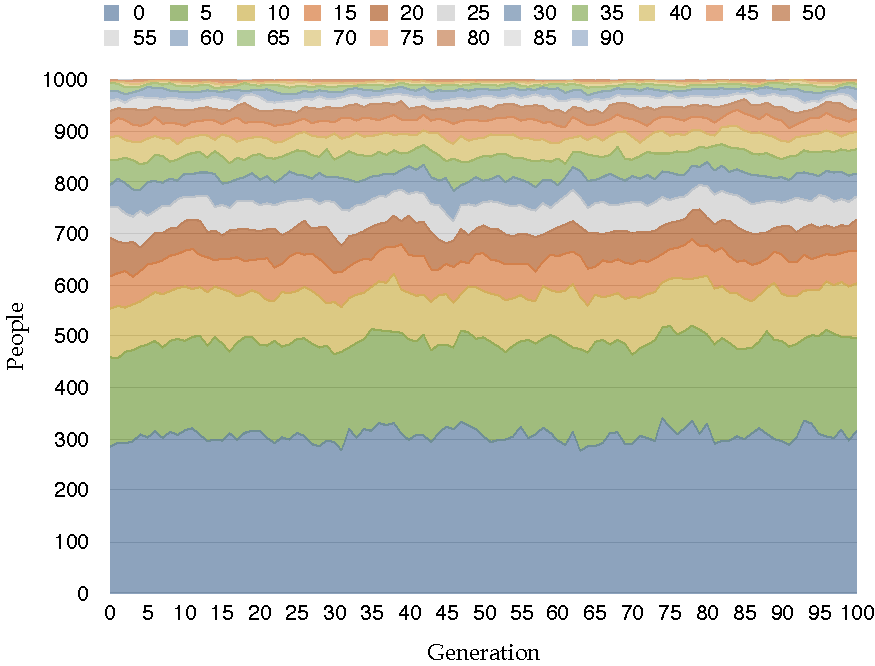
\includegraphics[width=\textwidth]{map_age_data}
\caption{Typical MAP simulation age structure}
\label{fig:mapResultsGraph}
\end{figure}

\begin{table}[h]
\caption{MAP Age Structures}
\label{tbl:mypAge}
\begin{tabular}{c c c c c c c}
\textbf{Age} & \textbf{Mean} & \textbf{Variance} & \textbf{Median} & \textbf{Minimum} & \textbf{Maximum} & \textbf{Range} \\\hline
0 & 308.00 & 179.576 & 307 & 278 & 342 & 64 \\\hline
5 & 183.48 & 139.949 & 182 & 159 & 207 & 48 \\\hline
10 & 95.41 & 81.759 & 94 & 71 & 124 & 53 \\\hline
15 & 63.39 & 60.867 & 66 & 45 & 88 & 43 \\\hline
20 & 57.29 & 53.097 & 56 & 40 & 76 & 36 \\\hline
25 & 53.64 & 53.687 & 53 & 38 & 71 & 33 \\\hline
30 & 48.79 & 51.077 & 48 & 32 & 69 & 37 \\\hline
35 & 42.40 & 57.232 & 42 & 26 & 63 & 37 \\\hline
40 & 36.31 & 44.903 & 36 & 20 & 54 & 34 \\\hline
45 & 31.27 & 29.977 & 31 & 19 & 47 & 28 \\\hline
50 & 24.68 & 23.230 & 25 & 15 & 38 & 23 \\\hline
55 & 18.02 & 20.505 & 18 & 8 & 31 & 23 \\\hline
60 & 14.52 & 14.293 & 14 & 5 & 25 & 20 \\\hline
65 & 9.69 & 8.297 & 9 & 3 & 16 & 13 \\\hline
70 & 5.77 & 3.755 & 6 & 1 & 10 & 9 \\\hline
75 & 2.91 & 2.729 & 3 & 0 & 6 & 6 \\\hline
80 & 1.14 & 0.869 & 1 & 0 & 5 & 5 \\\hline
85 & 0.29 & 0.228 & 0 & 0 & 2 & 2 \\\hline
90 & 0 & 0 & 0 & 0 & 0 & 0
\end{tabular}
\end{table}

\begin{figure}[h]
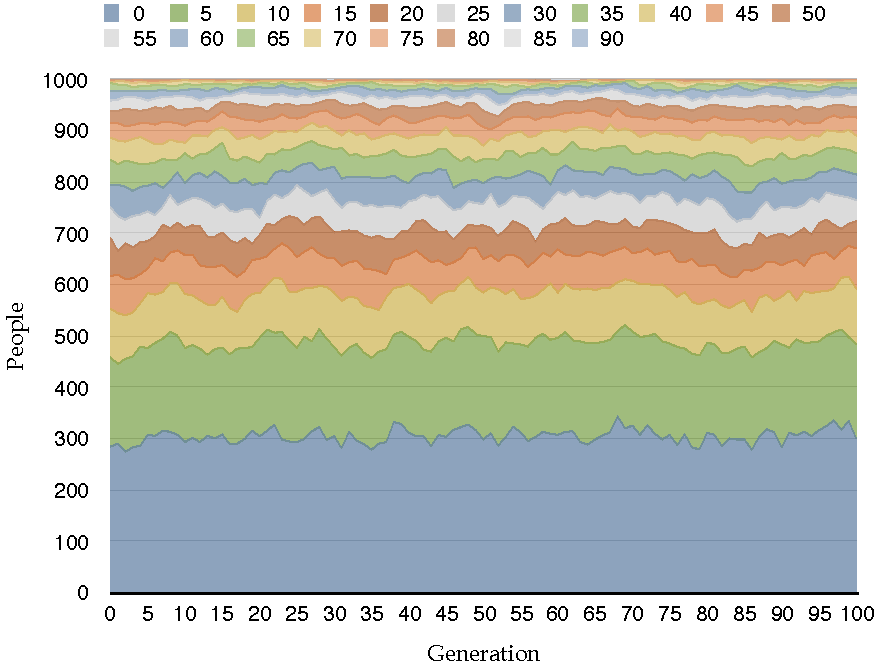
\includegraphics[width=\textwidth]{myp_age_data}
\caption{Typical MYP simulation age structure}
\label{fig:mypResultsGraph}
\end{figure}

\begin{table}[h]
\caption{MYP Age Structures}
\label{tbl:mypAge}
\begin{tabular}{c c c c c c c}
\textbf{Age} & \textbf{Mean} & \textbf{Variance} & \textbf{Median} & \textbf{Minimum} & \textbf{Maximum} & \textbf{Range} \\\hline
0 & 306.66 & 198.166 & 307 & 276 & 345 & 69 \\\hline
5 & 181.54 & 116.675 & 181.5 & 155 & 209 & 54 \\\hline
10 & 96.05 & 85.583 & 96 & 71 & 122 & 51 \\\hline
15 & 66.05 & 82.472 & 67 & 45 & 86 & 41 \\\hline
20 & 57.24 & 91.053 & 57.5 & 32 & 76 & 44 \\\hline
25 & 54.40 & 85.252 & 55 & 33 & 75 & 42 \\\hline
30 & 49.61 & 83.149 & 50 & 28 & 71 & 43 \\\hline
35 & 43.92 & 63.225 & 43 & 25 & 67 & 42 \\\hline
40 & 37.91 & 45.254 & 37 & 21 & 53 & 32 \\\hline
45 & 31.13 & 34.336 & 31 & 15 & 48 & 33 \\\hline
50 & 25.04 & 22.625 & 25 & 13 & 37 & 24 \\\hline
55 & 18.90 & 23.323 & 19 & 9 & 31 & 22 \\\hline
60 & 13.78 & 15.709 & 13.5 & 6 & 24 & 18 \\\hline
65 & 8.91 & 10.992 & 9 & 1 & 17 & 16 \\\hline
70 & 5.44 & 6.491 & 5 & 0 & 12 & 12 \\\hline
75 & 2.45 & 2.533 & 2 & 0 & 6 & 6 \\\hline
80 & 0.80 & 0.808 & 1 & 0 & 3 & 3 \\\hline
85 & 0.17 & 0.223 & 0 & 0  & 3 & 3 \\\hline
90 & 0 & 0 & 0 & 0 & 0 & 0
\end{tabular}
\end{table}



\begin{framed}
Sample output - maybe some graphs
What could have been done better - achieved with more work/time
\end{framed}

\chapter{Conclusion}
\label{cha:Conclusion}
Suggestions for further work.

\bibliographystyle{plain}
\bibliography{project} 

\appendix
\section{Typical MAP Run Results}
\label{adx:typicalMapResults}


\section{Typical MYP Run Results}
\label{adx:typicalMapResults}
\end{document}
